Sphericity matrix is defined using a collection of momenta $\vec{p}_i$, as \cite{BaBar:2014omp}:
\begin{equation}
    S^{\alpha,\beta} = \frac{\sum^N_{i=1}p_i^{\alpha}p_i^{\beta}}{\sum^N_{i=1}|\vec{p}_i|^2},
\end{equation}
where $\alpha,\beta\in\{x,y,z\}$.
For an isotropic distribution its three eigenvalues, $\lambda_{1-3}$, are expected to be of similar size.
On the other hand, collimated distributions tend to have one of the values significantly smaller.
Therefore two values are tested in this analysis as continuum suppression features:
\begin{itemize}
    \item $\mathtt{sphericity}\equiv\frac{3}{2}(\lambda_2+\lambda_3)\in(0,1)$ (\Cref{fig:sphericity});
    \item $\mathtt{aplanarity}\equiv\frac{3}{2}\lambda_3\in(0,1)$ (\Cref{fig:aplanarity}).
\end{itemize}
In these definitions, $\lambda_{3(2)}$ is the (second-)smallest eigenvalue of the sphericity matrix.
A spherical event will have a \texttt{sphericity} close to $1$, and \texttt{aplanarity} close to $1/2$.
As the definitions of the sphericity matrix include momentum, these variables turn out to introduce a significant bias to the photon energy spectrum and are therefore not used.

\begin{figure}[htbp!]
    \subcaptionbox{\label{fig:sphericity}}{
        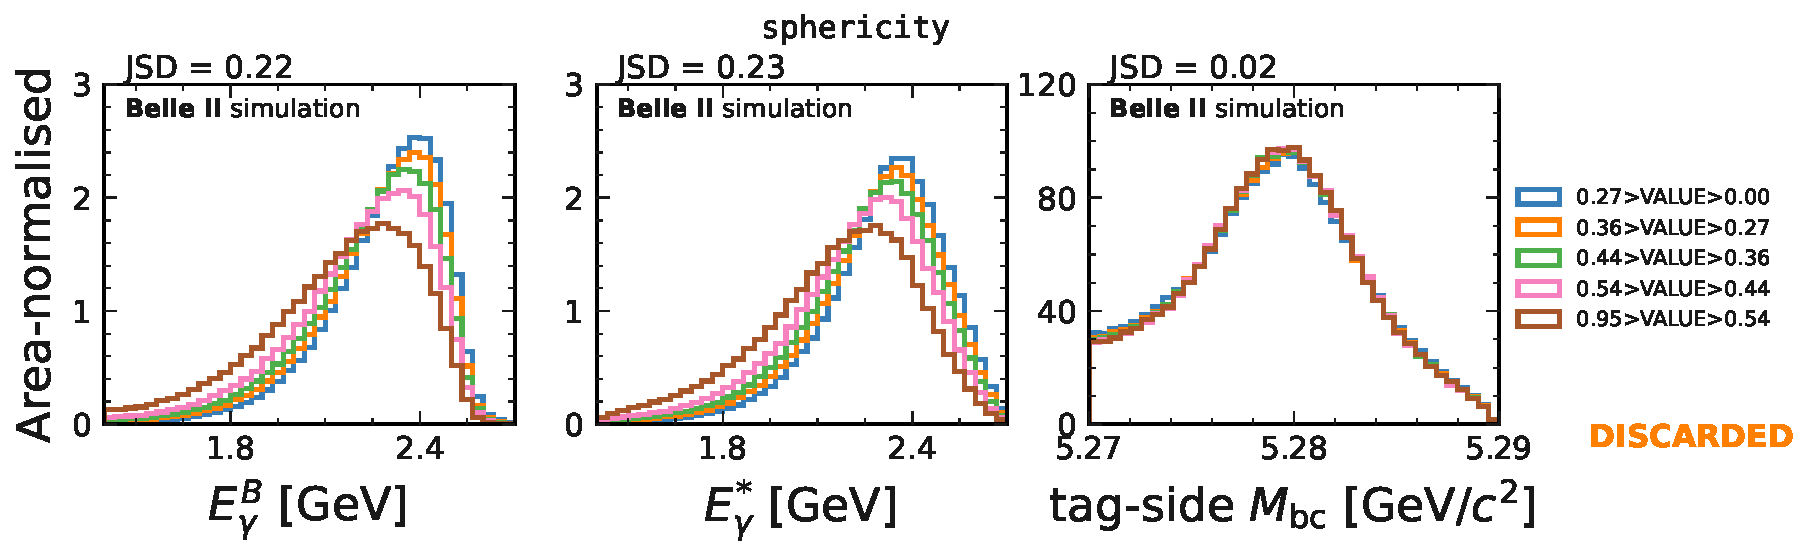
\includegraphics[width=0.95\textwidth]{figures/appendices/continuum_suppression_features/sphericity_aplanarity/sphericity_bias_tested.pdf}
    }
    \subcaptionbox{\label{fig:aplanarity}}{
        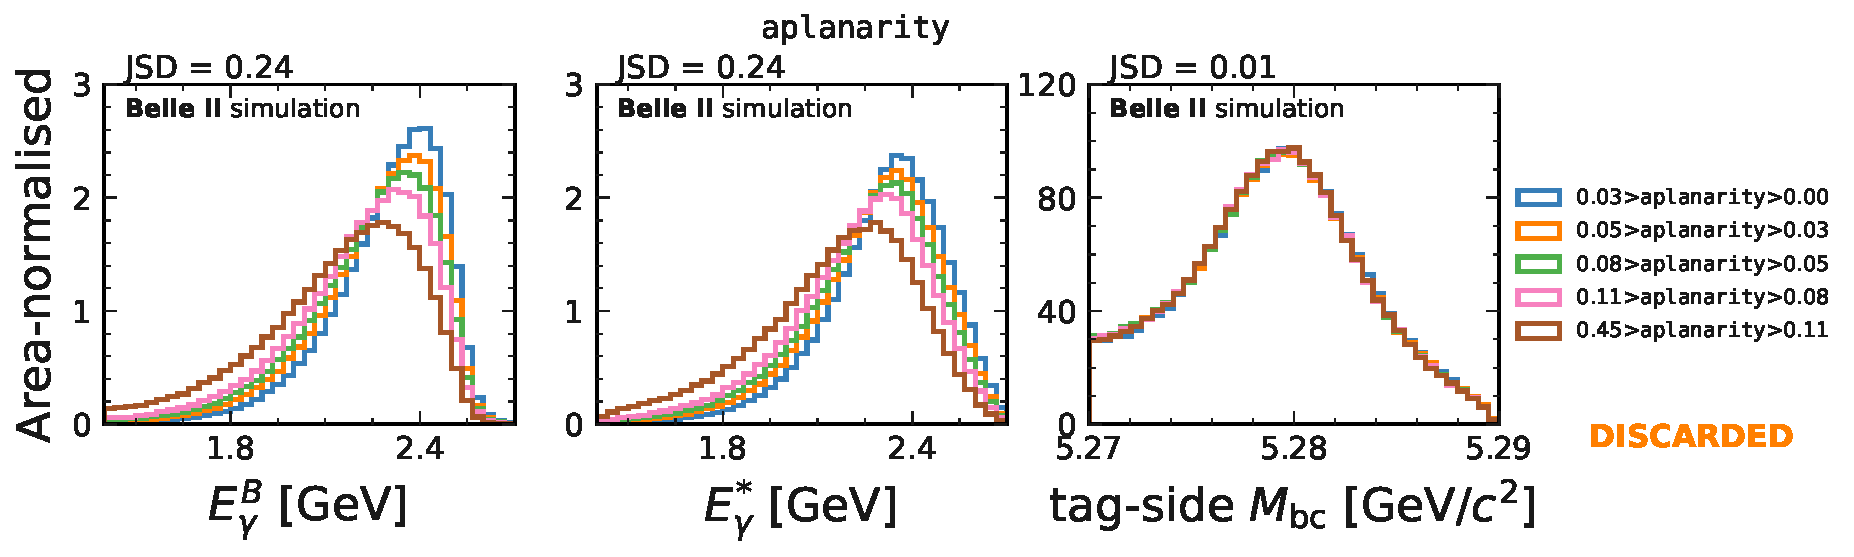
\includegraphics[width=0.95\textwidth]{figures/appendices/continuum_suppression_features/sphericity_aplanarity/aplanarity_bias_tested.pdf}

    }
    \caption{\label{fig:sphericity_aplanarity} The bias-test on \EB, \Estar and \Mbc for sphericity and aplanarity.
    The test is performed based on \textbf{Test~1} strategy, defined in \Cref{sec:continuum_features}.
    Variable definitions are given in the text.}
\end{figure}